\chapter{Laboratorio 2}
\section{Introduzione}
Nell'esperienza di laboratorio precedente, si è realizzato un circuito a guadagno unitario che realizza una funzione di buffer, con idealmente una resistenza di ingresso tendente ad infinito e una resistenza di uscita tendente a zero. In questa esperienza di laboratorio, si sono inizialmente effettuate ulteriori considerazioni sul circuito \textit{emitter follower} per poi realizzarne una versione \textit{single-ended}.

\section{Emitter follower: grafico ingresso-uscita}
Di seguito vengono riportati i risultati delle misure effettuate sul circuito precedentemente realizzato quando in ingresso è stato applicato un segnale sinusoidale con frequenza pari a \SI{1}{\kilo\hertz} e tensione picco-picco variabile da \SI{0.5}{\volt} a \SI{5}{\volt} con step di \SI{0.5}{\volt}. Si sono misurate le tensioni picco-picco in ingresso Vpp\sub{i} e in uscita Vpp\sub{o} al circuito grazie alle funzioni di misura integrate nell'oscilloscopio. Per rendere stabile il valore misurato, riducendo gli effetti del rumore e dei disturbi, è stato selezionato un filtro a \SI{20}{\mega\hertz} sugli ingressi dell'oscilloscopio e sono state effettuate delle medie (di 64 campioni) sui segnali. In questo modo è stato possibile ottenere un segnale meno rumoroso (\Fig\ref{fig:emitterfollwer_misurepiccopicco}).
\begin{table}[h!]
	\centering
	\begin{tabular}{c|c}
		\hline
		Vpp\sub{i} [V] & Vpp\sub{o} [V]\\ \hline
		0.509 & 0.491 \\ \hline
		1.019 & 0.984 \\ \hline
		1.502 & 1.476 \\ \hline
		2.080 & 1.994 \\ \hline
		2.565 & 2.474 \\ \hline
		3.037 & 2.962 \\ \hline
		3.524 & 3.459 \\ \hline
		4.022 & 3.967 \\ \hline
		4.606 & 4.470 \\ \hline
		5.089 & 4.945 \\ \hline
	\end{tabular}
	\caption{Valori picco-picco dei segnali misurati in ingresso del circuito (Vpp\sub{i}) e in uscita Vpp\sub{o}.}
	\label{tab:misurepiccopicco}
\end{table}
\begin{figure}[h!]
	\centering
	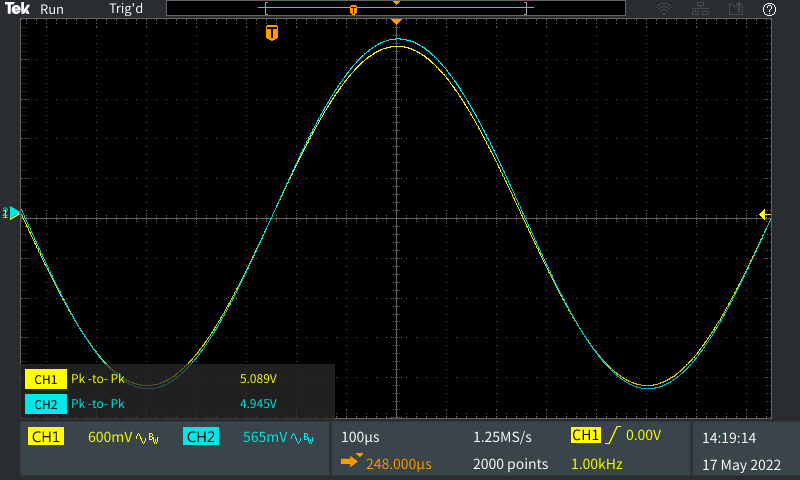
\includegraphics[width=0.7\linewidth]{./ImageFiles/Laboratorio 2/TEK00012}
	\caption{Misurazione della tensione picco-picco del segnale in ingresso (CH1) e in uscita (CH2) con i relativi valori picco-picco ricavati dall'oscilloscopio.}
	\label{fig:emitterfollwer_misurepiccopicco}
\end{figure}

\noindent
Come si può notare nella tabella \ref{tab:misurepiccopicco}, il valore del guadagno del circuito è leggermente inferiore a uno. Cerchiamo di quantificare il guadagno effettivo del circuito, confrontandolo con il valore teorico. Per fare ciò, è possibile rappresentare su un grafico il valore picco-picco di tensione misurato all'uscita del circuito in funzione della tensione in ingresso (ossia i valori riportati nella tabella precedente) ed eseguire un'interpolazione lineare della retta $y=a+bx$ che approssimi i valori ottenuti. Idealmente, vorremmo ottenere $a=1$ e $b=0$. Infatti, il coefficiente angolare della retta rappresenta il guadagno del circuito mentre l'intercetta un eventuale offset tra segnale in ingresso e uscita. Nella figura \ref{fig:emitterfollwer_inout} viene mostrato il risultato della retta interpolata sui dati stimata grazie alla funzione \textit{fitlm} offerta da Matlab. La retta identificata è $Vpp_o=-0.009+0.977\,Vpp_i$. Come si poteva già intuire osservando i dati nella tabella, si ottiene un guadagno leggermente inferiore a uno e un offset quasi nullo. Infatti, bisogna considerare che il circuito si comporta in uscita come un generatore di tensione reale e quindi con una resistenza di uscita finita, che influisce sulla tensione in uscita.
\begin{figure}[h!]
	\centering
	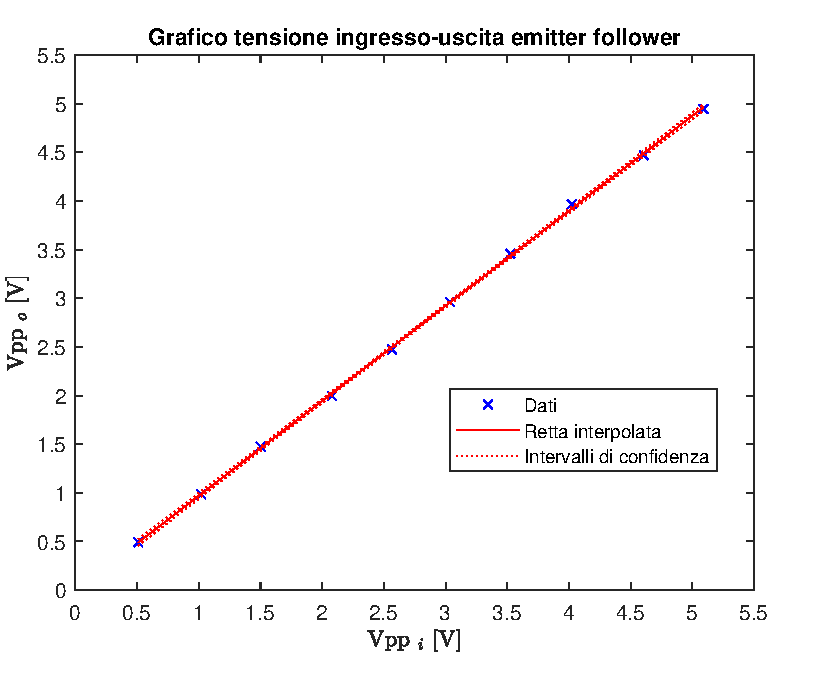
\includegraphics[width=0.7\linewidth]{./OtherFiles/Laboratorio 2/emitter follower-ingresso_uscita}
	\caption{Grafico ingresso-uscita del circuito emitter-follower (valori picco-picco delle tensioni misurate).}
	\label{fig:emitterfollwer_inout}
\end{figure}

\section{Emitter follower single-ended: prima versione}
Si vuole ora modificare il circuito precedente in modo da alimentarlo tra alimentazione positiva e massa, senza la necessità di utilizzare una alimentazione negativa. \`E stata realizzata una prima versione del circuito:
\begin{figure}[h!]
	\centering
	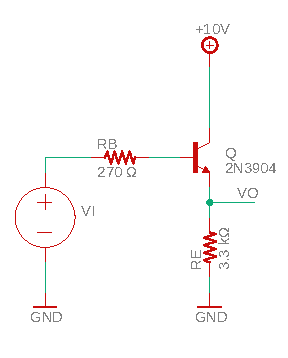
\includegraphics[width=0.4\linewidth]{./OtherFiles/Laboratorio 2/emitter follower}
	\caption{Schematico della prima versione del circuito emitter follower single-ended.}
	\label{fig:emitterfollwer_se}
\end{figure}

\noindent
Tuttavia, questo circuito presenta un problema. Dopo aver alimentato il circuito, applicando un segnale in ingresso v\sub{i} con frequenza di \SI{1}{\kilo\hertz} e tensione picco-picco di \SI{4}{\volt}, si nota che non funziona correttamente. Per capire meglio il comportamento del circuito è necessario analizzarne il punto di lavoro (\Fig\ref{fig:emitterfollwer_se_DC}), supponendo che il transistor sia in zona attiva diretta e con un $\beta\to\infty$ (che implica una corrente di base nulla).
\begin{figure}[h!]
	\centering
	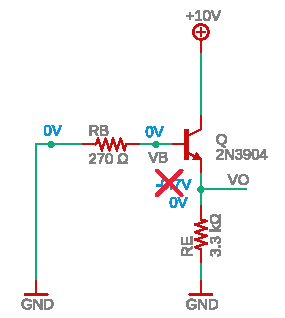
\includegraphics[width=0.4\linewidth]{./OtherFiles/Laboratorio 2/emitter follower_punto di lavoro-printout}
	\caption{Analisi punto di lavoro del circuito emitter follower single-ended.}
	\label{fig:emitterfollwer_se_DC}
\end{figure}

\noindent
La tensione al nodo V\sub{B} è di \SI{0}{\volt}, poiché non c'è caduta di potenziale in una resistenza attraversata da corrente nulla. Dalle ipotesi fatte, se ne deduce che la tensione al nodo V\sub{o} dovrebbe essere pari a \SI{-0.7}{\volt} (caduta di tensione giunzione base-emettitore). Tuttavia, se così fosse, nella resistenza R\sub{E} scorrerebbe una corrente da massa verso V\sub{o}. Questo però non è possibile: infatti, la corrente dovrebbe poi fluire nel transistor dall'emettitore. Per costruzione, non è però possibile avere una corrente entrante dall'emettitore di un transistor bipolare. Per questo motivo, l'unica soluzione ammissibile è che la corrente che attraversa la resistenza sia nulla e che il circuito sia spento: il nodo V\sub{o} di trova a una tensione di \SI{0}{\volt}. 

\noindent
Tuttavia, quando applichiamo un segnale sulla base con ampiezza maggiore di \SI{0.7}{\volt}, il circuito si accende (\Fig\ref{fig:emitterfollwer_se_statocircuito}). Infatti, il nodo V\sub{o} si porta a una tensione maggiore di \SI{0}{\volt} e il transistor è polarizzato correttamente.
\begin{figure}[h!]
	\centering
	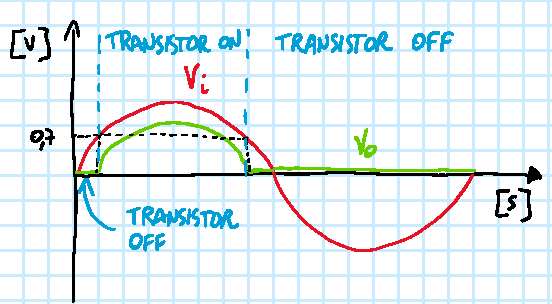
\includegraphics[width=0.7\linewidth]{./ImageFiles/Laboratorio 2/emitter follower errore soglia}
	\caption{Rappresentazione dello stato del circuito in funzione della tensione in ingresso.}
	\label{fig:emitterfollwer_se_statocircuito}
\end{figure}

\noindent
Questo comportamento anomalo è stato verificato sul circuito reale utilizzando l'oscilloscopio per visualizzare la tensione in ingresso e in uscita al circuito, come mostrato in figura \ref{fig:emitterfollwer_se_errore}.
\begin{figure}[h!]
	\centering
	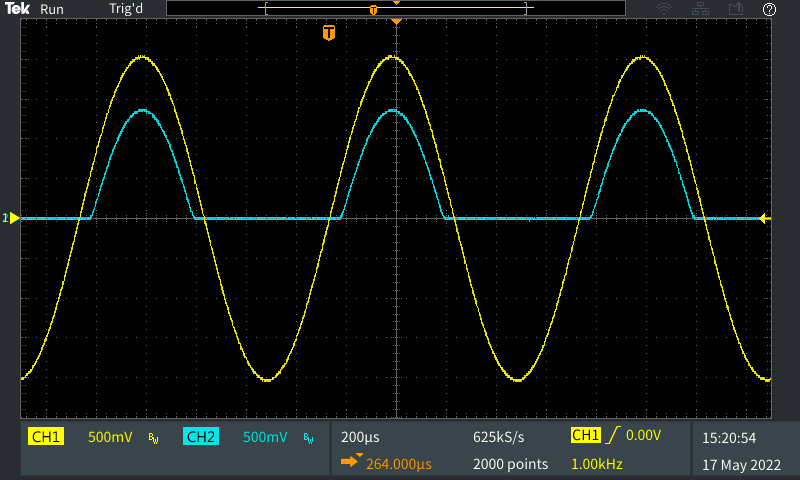
\includegraphics[width=0.7\linewidth]{./ImageFiles/Laboratorio 2/TEK00020}
	\caption{Tensione in ingresso (CH1) e in uscita (CH2) del circuito emitter follower single-ended. L'onda sinusoidale in ingresso ha una tensione picco-picco di \SI{4}{\volt} e frequenza \SI{1}{\kilo\hertz}.}
	\label{fig:emitterfollwer_se_errore}
\end{figure}

\noindent
Per ottenere il comportamento desiderato, è necessario inserire un offset di nel segnale in ingresso in modo che il transistor sia sempre polarizzato correttamente lungo tutto il periodo della sinusoide.

\section{Emitter follower single-ended: seconda versione}
Per garantire la corretta polarizzazione del transistor, è stato inserito un partitore di tensione realizzato con le resistenze R\sub{1} e R\sub{2} rispettivamente di valore \SI{130}{\kilo\ohm} e \SI{150}{\kilo\ohm} (\Fig\ref{fig:emitterfollwer_v2}). In questo modo, supponendo la corrente di base nulla (ossia $\beta\to\infty$), la tensione V\sub{B} è:
\begin{equation}
	V_B= \SI{10}{\volt}*\frac{R_2}{R_2+R_1}
	=\SI{10}{\volt}*\frac{\SI{150}{\kilo\ohm}}{\SI{150}{\kilo\ohm}+\SI{130}{\kilo\ohm}}\simeq\SI{5.357}{\volt}
	\label{eq:1}
\end{equation}
\begin{figure}[h!]
	\centering
	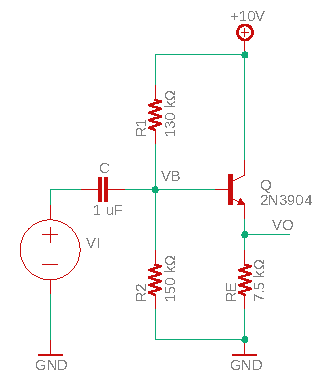
\includegraphics[width=0.4\linewidth]{./OtherFiles/Laboratorio 2/emitter follower_v2}
	\caption{Schematico della seconda versione del circuito emitter follower single-ended.}
	\label{fig:emitterfollwer_v2}
\end{figure}

\noindent
Tuttavia, è necessario inserire il condensatore C tra v\sub{i} e V\sub{B} in modo da disaccoppiare in continua i due nodi. Se non si inserisse un condensatore, il generatore v\sub{i} porterebbe la tensione al nodo V\sub{B} a massa nell'analisi del punto di lavoro, riportando il circuito nella situazione precedente.

\section{Componenti e misure}
Per realizzare il circuito in laboratorio (\Fig\ref{fig:emitterfollwer_v2_circuito}), si sono utilizzati i seguenti componenti:
\begin{itemize}
	\item transistor 2N3904;
	\item tre resistenze rispettivamente da R\sub{11}=\SI{12}{\kilo\ohm}, R\sub{12}=\SI{39}{\kilo\ohm} e R\sub{13}=\SI{82}{\kilo\ohm} connesse in serie per realizzare la resistenza R\sub{1};
	\item tre resistenze rispettivamente da R\sub{21}=\SI{39}{\kilo\ohm}, R\sub{22}=\SI{39}{\kilo\ohm} e R\sub{23}=\SI{82}{\kilo\ohm} connesse in serie per realizzare la resistenza R\sub{2};
	\item due resistenze rispettivamente da R\sub{E1}=\SI{3.9}{\kilo\ohm}, R\sub{E2}=\SI{3.9}{\kilo\ohm} connesse in serie per realizzare la resistenza R\sub{E};
	\item condensatore C da \SI{1}{\micro\farad}.
\end{itemize}
\begin{figure}[h!]
	\centering
	\includegraphics[width=0.5\linewidth]{./ImageFiles/Laboratorio 2/IMG\_20220517\_122529}
	\caption{Foto del circuito realizzato in laboratorio. \`E possibile notare anche i terminali per l'applicazione del segnale a un capo del condensatore.}
	\label{fig:emitterfollwer_v2_circuito}
\end{figure}

\noindent
Inoltre, sono stati utilizzati i seguenti strumenti:
\begin{itemize}
	\item alimentatore da banco con tensione positiva \SI{10}{\volt} e limite in corrente di \SI{50}{\milli\ampere};
	\item oscilloscopio a due canali;
	\item generatore di forme d'onda;
	\item multimetro da banco.
\end{itemize}

\noindent
Prima di utilizzare i componenti, si sono misurati i valori delle resistenze e delle giunzioni P-N del transistor utilizzato grazie al multimetro. Nella seguente tabella si riportano i risultati ottenuti:
\begin{table}[h!]
	\centering
	\begin{tabular}{c|c|c}
		\hline
		Componente & Valore nominale & Valore misurato \\ \hline
		R\sub{11} &\SI{12}{\kilo\ohm} & \SI{11.9}{\kilo\ohm} \\ \hline
		R\sub{12} &\SI{39}{\kilo\ohm} & \SI{39.0}{\kilo\ohm} \\ \hline
		R\sub{13} &\SI{82}{\kilo\ohm} & \SI{82.1}{\kilo\ohm} \\ \hline
		R\sub{21} &\SI{39}{\kilo\ohm} & \SI{37.8}{\kilo\ohm} \\ \hline
		R\sub{22} &\SI{39}{\kilo\ohm} & \SI{38.8}{\kilo\ohm} \\ \hline
		R\sub{23} &\SI{82}{\kilo\ohm} & \SI{82.2}{\kilo\ohm} \\ \hline
		R\sub{E1} &\SI{3.9}{\kilo\ohm} & \SI{3.9}{\kilo\ohm} \\ \hline
		R\sub{E2} &\SI{3.9}{\kilo\ohm} & \SI{3.8}{\kilo\ohm} \\ \hline
		Vd\sub{B-E} & $\simeq$ \SI{0.7}{\volt} & \SI{0.700}{\volt} \\ \hline
		Vd\sub{B-C} & $\simeq$ \SI{0.7}{\volt} & \SI{0.679}{\volt} \\ \hline
	\end{tabular}
\end{table}

\noindent
L'analisi del punto stazionario e di piccolo segnale possono essere facilmente ricavate dalle analisi precedenti. In particolare, nell'analisi di piccolo segnale è sufficiente considerare il condensatore come un corto. Di conseguenza $v_b=v_i$ e l'analisi prosegue come nel circuito precedente. Per quanto riguarda l'analisi del punto di lavoro, otteniamo il circuito rappresentato in figura \ref{fig:emitterfollwer_v2_DC}. 
\begin{figure}[h!]
	\centering
	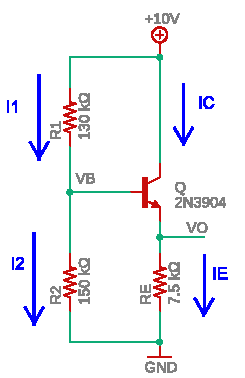
\includegraphics[width=0.4\linewidth]{./OtherFiles/Laboratorio 2/emitter follower_v2_punto di lavoro-printout}
	\caption{Analisi punto di lavoro del circuito emitter follower single-ended (seconda versione).}
	\label{fig:emitterfollwer_v2_DC}
\end{figure}
Il condensatore disaccoppia in DC i nodi ai suoi capi. Quindi viene considerato come un circuito aperto. Inoltre, se si considera la corrente di base nulla ($\beta\to\infty$), la corrente I\sub{1} è uguale alla corrente I\sub{2}. Utilizzando l'equazione \ref{eq:1} del partitore di tensione, è possibile ricavare la tensione V\sub{o}. Ipotizzando il transistor in regione attiva diretta, la tensione V\sub{o} sarà $V_o=V_B-\SI{0.7}{\volt}\simeq\SI{5.357}{\volt}-\SI{0.7}{\volt}=\SI{4.657}{\volt}$. Inoltre, facendo un bilancio di correnti nel transistor, si ottiene:
\begin{equation}
	\begin{split}
		I_C&=I_E \\
		&=\frac{V_o-\SI{0}{\volt}}{R_E} \\
		&=\frac{\SI{4.657}{\volt}}{\SI{7.5}{\kilo\ohm}}=\SI{0.6209}{\milli\ampere}
	\end{split}
\end{equation}
\`E verificata anche l'ipotesi che il transistor si trovi in regione attiva diretta, in quanto $V_{CE}>0$.

Una volta realizzato il circuito, sono state misurate dapprima le tensioni V\sub{E} e V\sub{B} con il nodo V\sub{i} a massa. Da queste, è possibile ricavare le correnti I\sub{1}, I\sub{2} e I\sub{E} tramite la legge di Ohm. Infine, è possibile calcolare la corrente di base come $I_B=I_1-I_2$ (bilancio delle correnti al nodo V\sub{B}) e la corrente di collettore $I_C=I_E-I_B$.
Sono stati ottenuti i seguenti valori:
\begin{table}[h!]
	\centering
	\begin{tabular}{c|c|c|c|c|c|c}
		\hline
		V\sub{o} [V] & V\sub{B} [V] & I\sub{1} [mA] & I\sub{2} [mA] & I\sub{E} [mA] & I\sub{B} [mA] & I\sub{C} [mA]\\ \hline
		4.556 & 5.172 & 0.0363 & 0.0326 & 0.5917 & 0.0037 & 0.5880 \\ \hline
	\end{tabular}
\end{table}

\noindent
Come si può osservare, le misure reali rispecchiano con buona approssimazione i valori attesi dall'analisi teorica. 

\noindent
In figura \ref{fig:emitterfollwer_v2_AC} sono rappresentati i segnali in ingresso (applicato al noto V\sub{i}) e in uscita (nodo V\sub{o}) al circuito. Il segnale applicato in ingresso è definito da una sinusoide di ampiezza \SI{2}{\volt} e frequenza \SI{1}{\kilo\hertz}. I due segnali hanno, con buona approssimazione, la medesima ampiezza e non è presente uno sfasamento. Il grafico XY (\Fig\ref{fig:emitterfollwer_v2_XY}) mostra un segmento, come aspettato in caso di segnali in fase.
\begin{figure}[h!]
	\centering
	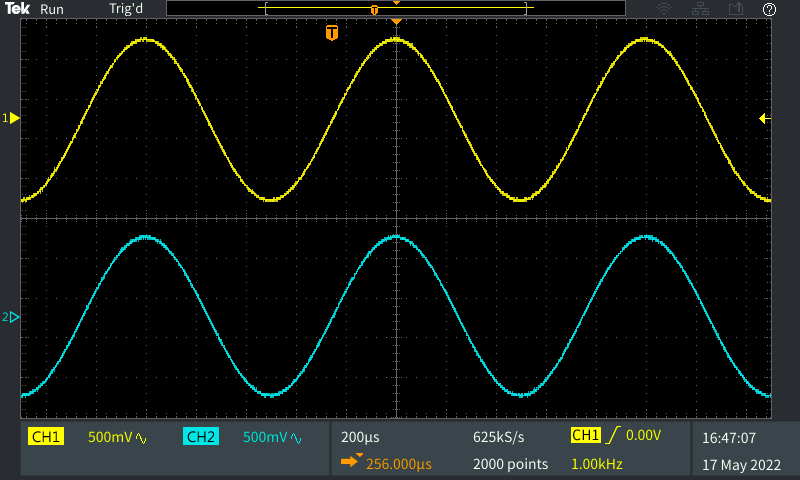
\includegraphics[width=0.8\linewidth]{./ImageFiles/Laboratorio 2/TEK00023}
	\caption{Confronto tra il segnale in ingresso (CH1) e in uscita (CH2) all'emitter follower.}
	\label{fig:emitterfollwer_v2_AC}
\end{figure}
\begin{figure}[h!]
	\centering
	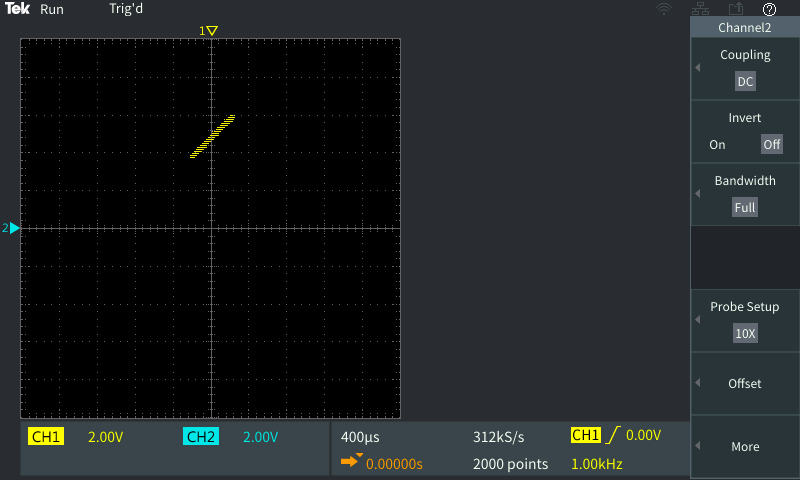
\includegraphics[width=0.8\linewidth]{./ImageFiles/Laboratorio 3/TEK00001}
	\caption{Grafico XY ingresso (CH1) e in uscita (CH2) all'emitter follower. L'onda applicata in ingresso è una sinusoide con ampiezza \SI{2}{\volt} e frequenza \SI{1}{\kilo\hertz}.}
	\label{fig:emitterfollwer_v2_XY}
\end{figure}